\documentclass{standalone}
\usepackage{tikz}
\usetikzlibrary{patterns, positioning}

\begin{document}
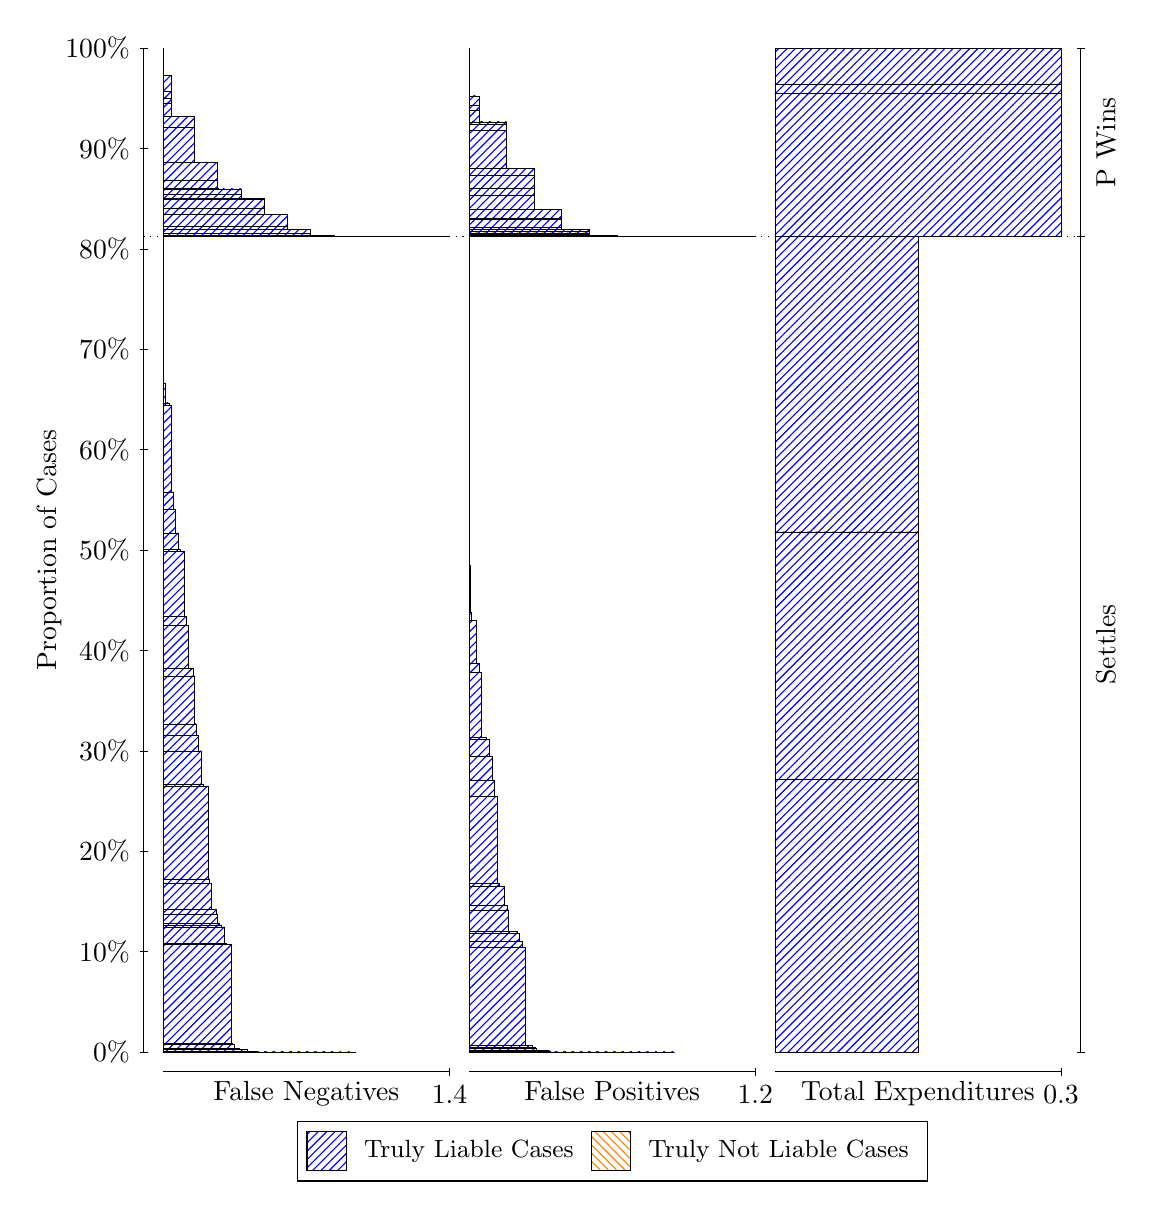
\begin{tikzpicture}
\draw[black, very thin] (1.5,1.75) -- (1.5,14.5);
\node[rotate=90, anchor=center] at (0.3, 8.125) {Proportion of Cases};
\draw[black, very thin] (1.45,1.75) -- (1.55,1.75);
\node[anchor=east] at (1.45, 1.75) {0\%};
\draw[black, very thin] (1.45,3.025) -- (1.55,3.025);
\node[anchor=east] at (1.45, 3.025) {10\%};
\draw[black, very thin] (1.45,4.3) -- (1.55,4.3);
\node[anchor=east] at (1.45, 4.3) {20\%};
\draw[black, very thin] (1.45,5.575) -- (1.55,5.575);
\node[anchor=east] at (1.45, 5.575) {30\%};
\draw[black, very thin] (1.45,6.85) -- (1.55,6.85);
\node[anchor=east] at (1.45, 6.85) {40\%};
\draw[black, very thin] (1.45,8.125) -- (1.55,8.125);
\node[anchor=east] at (1.45, 8.125) {50\%};
\draw[black, very thin] (1.45,9.4) -- (1.55,9.4);
\node[anchor=east] at (1.45, 9.4) {60\%};
\draw[black, very thin] (1.45,10.675) -- (1.55,10.675);
\node[anchor=east] at (1.45, 10.675) {70\%};
\draw[black, very thin] (1.45,11.95) -- (1.55,11.95);
\node[anchor=east] at (1.45, 11.95) {80\%};
\draw[black, very thin] (1.45,13.225) -- (1.55,13.225);
\node[anchor=east] at (1.45, 13.225) {90\%};
\draw[black, very thin] (1.45,14.5) -- (1.55,14.5);
\node[anchor=east] at (1.45, 14.5) {100\%};

\draw[black, very thin] (13.4,1.75) -- (13.4,14.5);
\draw[black, very thin] (13.35,1.75) -- (13.45,1.75);
\node[anchor=west] at (13.35, 1.75) {};
\draw[black, very thin] (13.35,12.104) -- (13.45,12.104);
\node[anchor=west] at (13.35, 12.104) {};
\draw[black, very thin] (13.35,14.5) -- (13.45,14.5);
\node[anchor=west] at (13.35, 14.5) {};

\draw[black, very thin, pattern color=blue, pattern=north east lines] (1.75,1.75) rectangle (4.1942,1.75);
\draw[black, very thin, pattern color=blue, pattern=north east lines] (1.75,1.75) rectangle (3.93,1.75);
\draw[black, very thin, pattern color=blue, pattern=north east lines] (1.75,1.75) rectangle (3.9006,1.75);
\draw[black, very thin, pattern color=blue, pattern=north east lines] (1.75,1.75) rectangle (3.7979,1.75);
\draw[black, very thin, pattern color=blue, pattern=north east lines] (1.75,1.75) rectangle (3.6658,1.75);
\draw[black, very thin, pattern color=blue, pattern=north east lines] (1.75,1.75) rectangle (3.6364,1.75);
\draw[black, very thin, pattern color=blue, pattern=north east lines] (1.75,1.75) rectangle (3.607,1.75);
\draw[black, very thin, pattern color=blue, pattern=north east lines] (1.75,1.75) rectangle (3.5336,1.75);
\draw[black, very thin, pattern color=blue, pattern=north east lines] (1.75,1.75) rectangle (3.5043,1.75);
\draw[black, very thin, pattern color=blue, pattern=north east lines] (1.75,1.75) rectangle (3.4015,1.75);
\draw[black, very thin, pattern color=blue, pattern=north east lines] (1.75,1.75) rectangle (3.3722,1.75);
\draw[black, very thin, pattern color=blue, pattern=north east lines] (1.75,1.75) rectangle (3.3428,1.75);
\draw[black, very thin, pattern color=blue, pattern=north east lines] (1.75,1.75) rectangle (3.3134,1.75);
\draw[black, very thin, pattern color=blue, pattern=north east lines] (1.75,1.75) rectangle (3.24,1.75);
\draw[black, very thin, pattern color=blue, pattern=north east lines] (1.75,1.75) rectangle (3.2107,1.75);
\draw[black, very thin, pattern color=blue, pattern=north east lines] (1.75,1.75) rectangle (3.1373,1.75);
\draw[black, very thin, pattern color=blue, pattern=north east lines] (1.75,1.75) rectangle (3.1079,1.7506);
\draw[black, very thin, pattern color=blue, pattern=north east lines] (1.75,1.7506) rectangle (3.0786,1.7506);
\draw[black, very thin, pattern color=blue, pattern=north east lines] (1.75,1.7506) rectangle (3.0492,1.7506);
\draw[black, very thin, pattern color=blue, pattern=north east lines] (1.75,1.7506) rectangle (3.0198,1.7507);
\draw[black, very thin, pattern color=blue, pattern=north east lines] (1.75,1.7507) rectangle (3.0052,1.7511);
\draw[black, very thin, pattern color=blue, pattern=north east lines] (1.75,1.7511) rectangle (2.9464,1.7536);
\draw[black, very thin, pattern color=blue, pattern=north east lines] (1.75,1.7536) rectangle (2.9171,1.7538);
\draw[black, very thin, pattern color=blue, pattern=north east lines] (1.75,1.7538) rectangle (2.8437,1.7541);
\draw[black, very thin, pattern color=blue, pattern=north east lines] (1.75,1.7541) rectangle (2.8143,1.7782);
\draw[black, very thin, pattern color=blue, pattern=north east lines] (1.75,1.7782) rectangle (2.7849,1.7787);
\draw[black, very thin, pattern color=blue, pattern=north east lines] (1.75,1.7787) rectangle (2.7556,1.7792);
\draw[black, very thin, pattern color=blue, pattern=north east lines] (1.75,1.7792) rectangle (2.7262,1.7849);
\draw[black, very thin, pattern color=blue, pattern=north east lines] (1.75,1.7849) rectangle (2.7115,1.7924);
\draw[black, very thin, pattern color=blue, pattern=north east lines] (1.75,1.7924) rectangle (2.6528,1.8506);
\draw[black, very thin, pattern color=blue, pattern=north east lines] (1.75,1.8506) rectangle (2.6235,1.8575);
\draw[black, very thin, pattern color=blue, pattern=north east lines] (1.75,1.8575) rectangle (2.6088,3.1206);
\draw[black, very thin, pattern color=blue, pattern=north east lines] (1.75,3.1206) rectangle (2.5501,3.1261);
\draw[black, very thin, pattern color=blue, pattern=north east lines] (1.75,3.1261) rectangle (2.5207,3.3375);
\draw[black, very thin, pattern color=blue, pattern=north east lines] (1.75,3.3375) rectangle (2.4913,3.3609);
\draw[black, very thin, pattern color=blue, pattern=north east lines] (1.75,3.3609) rectangle (2.462,3.3815);
\draw[black, very thin, pattern color=blue, pattern=north east lines] (1.75,3.3815) rectangle (2.4326,3.5027);
\draw[black, very thin, pattern color=blue, pattern=north east lines] (1.75,3.5027) rectangle (2.4179,3.5563);
\draw[black, very thin, pattern color=blue, pattern=north east lines] (1.75,3.5563) rectangle (2.3592,3.8903);
\draw[black, very thin, pattern color=blue, pattern=north east lines] (1.75,3.8903) rectangle (2.3299,3.9486);
\draw[black, very thin, pattern color=blue, pattern=north east lines] (1.75,3.9486) rectangle (2.3152,5.1245);
\draw[black, very thin, pattern color=blue, pattern=north east lines] (1.75,5.1245) rectangle (2.2565,5.1507);
\draw[black, very thin, pattern color=blue, pattern=north east lines] (1.75,5.1507) rectangle (2.2271,5.5742);
\draw[black, very thin, pattern color=blue, pattern=north east lines] (1.75,5.5742) rectangle (2.1977,5.7667);
\draw[black, very thin, pattern color=blue, pattern=north east lines] (1.75,5.7667) rectangle (2.1684,5.9173);
\draw[black, very thin, pattern color=blue, pattern=north east lines] (1.75,5.9173) rectangle (2.139,6.5235);
\draw[black, very thin, pattern color=blue, pattern=north east lines] (1.75,6.5235) rectangle (2.1243,6.6186);
\draw[black, very thin, pattern color=blue, pattern=north east lines] (1.75,6.6186) rectangle (2.0656,7.1644);
\draw[black, very thin, pattern color=blue, pattern=north east lines] (1.75,7.1644) rectangle (2.0363,7.2856);
\draw[black, very thin, pattern color=blue, pattern=north east lines] (1.75,7.2856) rectangle (2.0216,8.1057);
\draw[black, very thin, pattern color=blue, pattern=north east lines] (1.75,8.1057) rectangle (1.9629,8.1314);
\draw[black, very thin, pattern color=blue, pattern=north east lines] (1.75,8.1314) rectangle (1.9335,8.3432);
\draw[black, very thin, pattern color=blue, pattern=north east lines] (1.75,8.3432) rectangle (1.9041,8.6483);
\draw[black, very thin, pattern color=blue, pattern=north east lines] (1.75,8.6483) rectangle (1.8748,8.8621);
\draw[black, very thin, pattern color=blue, pattern=north east lines] (1.75,8.8621) rectangle (1.8454,9.9611);
\draw[black, very thin, pattern color=blue, pattern=north east lines] (1.75,9.9611) rectangle (1.8307,9.9937);
\draw[black, very thin, pattern color=blue, pattern=north east lines] (1.75,9.9937) rectangle (1.772,10.239);
\draw[black, very thin, pattern color=orange, pattern=north west lines] (1.75,10.239) rectangle (1.75,10.239);
\draw[black, very thin, pattern color=blue, pattern=north east lines] (1.75,10.239) rectangle (1.75,12.104);
\draw[black, very thin, pattern color=blue, pattern=north east lines] (1.75,12.104) rectangle (5.3833,12.104);
\draw[black, very thin, pattern color=blue, pattern=north east lines] (1.75,12.104) rectangle (5.0897,12.104);
\draw[black, very thin, pattern color=blue, pattern=north east lines] (1.75,12.104) rectangle (4.7961,12.104);
\draw[black, very thin, pattern color=blue, pattern=north east lines] (1.75,12.104) rectangle (4.5025,12.104);
\draw[black, very thin, pattern color=blue, pattern=north east lines] (1.75,12.104) rectangle (4.5025,12.104);
\draw[black, very thin, pattern color=blue, pattern=north east lines] (1.75,12.104) rectangle (4.2089,12.106);
\draw[black, very thin, pattern color=blue, pattern=north east lines] (1.75,12.106) rectangle (4.2016,12.106);
\draw[black, very thin, pattern color=blue, pattern=north east lines] (1.75,12.106) rectangle (3.9153,12.121);
\draw[black, very thin, pattern color=blue, pattern=north east lines] (1.75,12.121) rectangle (3.908,12.121);
\draw[black, very thin, pattern color=blue, pattern=north east lines] (1.75,12.121) rectangle (3.6217,12.15);
\draw[black, very thin, pattern color=blue, pattern=north east lines] (1.75,12.15) rectangle (3.6217,12.195);
\draw[black, very thin, pattern color=blue, pattern=north east lines] (1.75,12.195) rectangle (3.6144,12.195);
\draw[black, very thin, pattern color=blue, pattern=north east lines] (1.75,12.195) rectangle (3.6144,12.195);
\draw[black, very thin, pattern color=blue, pattern=north east lines] (1.75,12.195) rectangle (3.3281,12.238);
\draw[black, very thin, pattern color=blue, pattern=north east lines] (1.75,12.238) rectangle (3.3281,12.389);
\draw[black, very thin, pattern color=blue, pattern=north east lines] (1.75,12.389) rectangle (3.3208,12.39);
\draw[black, very thin, pattern color=blue, pattern=north east lines] (1.75,12.39) rectangle (3.0345,12.462);
\draw[black, very thin, pattern color=blue, pattern=north east lines] (1.75,12.462) rectangle (3.0345,12.583);
\draw[black, very thin, pattern color=blue, pattern=north east lines] (1.75,12.583) rectangle (3.0272,12.584);
\draw[black, very thin, pattern color=blue, pattern=north east lines] (1.75,12.584) rectangle (3.0272,12.589);
\draw[black, very thin, pattern color=blue, pattern=north east lines] (1.75,12.589) rectangle (2.7409,12.645);
\draw[black, very thin, pattern color=blue, pattern=north east lines] (1.75,12.645) rectangle (2.7336,12.712);
\draw[black, very thin, pattern color=blue, pattern=north east lines] (1.75,12.712) rectangle (2.4473,12.717);
\draw[black, very thin, pattern color=blue, pattern=north east lines] (1.75,12.717) rectangle (2.44,12.815);
\draw[black, very thin, pattern color=blue, pattern=north east lines] (1.75,12.815) rectangle (2.44,13.043);
\draw[black, very thin, pattern color=blue, pattern=north east lines] (1.75,13.043) rectangle (2.1537,13.043);
\draw[black, very thin, pattern color=blue, pattern=north east lines] (1.75,13.043) rectangle (2.1464,13.489);
\draw[black, very thin, pattern color=blue, pattern=north east lines] (1.75,13.489) rectangle (2.1464,13.636);
\draw[black, very thin, pattern color=blue, pattern=north east lines] (1.75,13.636) rectangle (1.8601,13.636);
\draw[black, very thin, pattern color=blue, pattern=north east lines] (1.75,13.636) rectangle (1.8528,13.802);
\draw[black, very thin, pattern color=blue, pattern=north east lines] (1.75,13.802) rectangle (1.8528,13.867);
\draw[black, very thin, pattern color=blue, pattern=north east lines] (1.75,13.867) rectangle (1.8528,13.949);
\draw[black, very thin, pattern color=blue, pattern=north east lines] (1.75,13.949) rectangle (1.8528,14.151);
\draw[black, very thin, pattern color=orange, pattern=north west lines] (1.75,14.151) rectangle (1.75,14.151);
\draw[black, very thin, pattern color=blue, pattern=north east lines] (1.75,14.151) rectangle (1.75,14.5);
\draw[black, very thin, pattern color=orange, pattern=north west lines] (5.6333,1.75) rectangle (8.2399,1.75);
\draw[black, very thin, pattern color=blue, pattern=north east lines] (5.6333,1.75) rectangle (8.2399,1.75);
\draw[black, very thin, pattern color=blue, pattern=north east lines] (5.6333,1.75) rectangle (7.8888,1.75);
\draw[black, very thin, pattern color=orange, pattern=north west lines] (5.6333,1.75) rectangle (7.7659,1.75);
\draw[black, very thin, pattern color=blue, pattern=north east lines] (5.6333,1.75) rectangle (7.7659,1.75);
\draw[black, very thin, pattern color=orange, pattern=north west lines] (5.6333,1.75) rectangle (7.608,1.75);
\draw[black, very thin, pattern color=blue, pattern=north east lines] (5.6333,1.75) rectangle (7.608,1.75);
\draw[black, very thin, pattern color=blue, pattern=north east lines] (5.6333,1.75) rectangle (7.5378,1.75);
\draw[black, very thin, pattern color=blue, pattern=north east lines] (5.6333,1.75) rectangle (7.4149,1.75);
\draw[black, very thin, pattern color=orange, pattern=north west lines] (5.6333,1.75) rectangle (7.292,1.75);
\draw[black, very thin, pattern color=blue, pattern=north east lines] (5.6333,1.75) rectangle (7.292,1.75);
\draw[black, very thin, pattern color=blue, pattern=north east lines] (5.6333,1.75) rectangle (7.2569,1.75);
\draw[black, very thin, pattern color=blue, pattern=north east lines] (5.6333,1.75) rectangle (7.1867,1.75);
\draw[black, very thin, pattern color=orange, pattern=north west lines] (5.6333,1.75) rectangle (7.1341,1.75);
\draw[black, very thin, pattern color=blue, pattern=north east lines] (5.6333,1.75) rectangle (7.1341,1.75);
\draw[black, very thin, pattern color=blue, pattern=north east lines] (5.6333,1.75) rectangle (7.0638,1.75);
\draw[black, very thin, pattern color=orange, pattern=north west lines] (5.6333,1.75) rectangle (6.9761,1.75);
\draw[black, very thin, pattern color=blue, pattern=north east lines] (5.6333,1.75) rectangle (6.9761,1.7501);
\draw[black, very thin, pattern color=blue, pattern=north east lines] (5.6333,1.7501) rectangle (6.941,1.7501);
\draw[black, very thin, pattern color=blue, pattern=north east lines] (5.6333,1.7501) rectangle (6.9059,1.7501);
\draw[black, very thin, pattern color=blue, pattern=north east lines] (5.6333,1.7501) rectangle (6.8357,1.7506);
\draw[black, very thin, pattern color=orange, pattern=north west lines] (5.6333,1.7506) rectangle (6.8181,1.7506);
\draw[black, very thin, pattern color=blue, pattern=north east lines] (5.6333,1.7506) rectangle (6.8181,1.7511);
\draw[black, very thin, pattern color=blue, pattern=north east lines] (5.6333,1.7511) rectangle (6.783,1.7517);
\draw[black, very thin, pattern color=blue, pattern=north east lines] (5.6333,1.7517) rectangle (6.7128,1.7517);
\draw[black, very thin, pattern color=orange, pattern=north west lines] (5.6333,1.7517) rectangle (6.6601,1.7517);
\draw[black, very thin, pattern color=blue, pattern=north east lines] (5.6333,1.7517) rectangle (6.6601,1.7626);
\draw[black, very thin, pattern color=blue, pattern=north east lines] (5.6333,1.7626) rectangle (6.625,1.7685);
\draw[black, very thin, pattern color=blue, pattern=north east lines] (5.6333,1.7685) rectangle (6.5899,1.769);
\draw[black, very thin, pattern color=blue, pattern=north east lines] (5.6333,1.769) rectangle (6.5548,1.7692);
\draw[black, very thin, pattern color=blue, pattern=north east lines] (5.6333,1.7692) rectangle (6.4846,1.7955);
\draw[black, very thin, pattern color=blue, pattern=north east lines] (5.6333,1.7955) rectangle (6.4671,1.8034);
\draw[black, very thin, pattern color=blue, pattern=north east lines] (5.6333,1.8034) rectangle (6.432,1.8294);
\draw[black, very thin, pattern color=blue, pattern=north east lines] (5.6333,1.8294) rectangle (6.3618,1.8314);
\draw[black, very thin, pattern color=orange, pattern=north west lines] (5.6333,1.8314) rectangle (6.3442,1.8314);
\draw[black, very thin, pattern color=blue, pattern=north east lines] (5.6333,1.8314) rectangle (6.3442,3.0836);
\draw[black, very thin, pattern color=blue, pattern=north east lines] (5.6333,3.0836) rectangle (6.3091,3.1604);
\draw[black, very thin, pattern color=blue, pattern=north east lines] (5.6333,3.1604) rectangle (6.274,3.2548);
\draw[black, very thin, pattern color=blue, pattern=north east lines] (5.6333,3.2548) rectangle (6.2389,3.2787);
\draw[black, very thin, pattern color=blue, pattern=north east lines] (5.6333,3.2787) rectangle (6.2038,3.2836);
\draw[black, very thin, pattern color=blue, pattern=north east lines] (5.6333,3.2836) rectangle (6.1336,3.5555);
\draw[black, very thin, pattern color=blue, pattern=north east lines] (5.6333,3.5555) rectangle (6.116,3.6146);
\draw[black, very thin, pattern color=blue, pattern=north east lines] (5.6333,3.6146) rectangle (6.0809,3.8602);
\draw[black, very thin, pattern color=blue, pattern=north east lines] (5.6333,3.8602) rectangle (6.0107,3.8929);
\draw[black, very thin, pattern color=blue, pattern=north east lines] (5.6333,3.8929) rectangle (5.9932,4.9918);
\draw[black, very thin, pattern color=blue, pattern=north east lines] (5.6333,4.9918) rectangle (5.9581,5.2057);
\draw[black, very thin, pattern color=blue, pattern=north east lines] (5.6333,5.2057) rectangle (5.9229,5.5108);
\draw[black, very thin, pattern color=blue, pattern=north east lines] (5.6333,5.5108) rectangle (5.8878,5.7225);
\draw[black, very thin, pattern color=blue, pattern=north east lines] (5.6333,5.7225) rectangle (5.8527,5.7483);
\draw[black, very thin, pattern color=blue, pattern=north east lines] (5.6333,5.7483) rectangle (5.7825,6.5683);
\draw[black, very thin, pattern color=blue, pattern=north east lines] (5.6333,6.5683) rectangle (5.765,6.6896);
\draw[black, very thin, pattern color=blue, pattern=north east lines] (5.6333,6.6896) rectangle (5.7299,7.2354);
\draw[black, very thin, pattern color=blue, pattern=north east lines] (5.6333,7.2354) rectangle (5.6597,7.3304);
\draw[black, very thin, pattern color=blue, pattern=north east lines] (5.6333,7.3304) rectangle (5.6421,7.9366);
\draw[black, very thin, pattern color=blue, pattern=north east lines] (5.6333,7.9366) rectangle (5.6333,12.104);
\draw[black, very thin, pattern color=orange, pattern=north west lines] (5.6333,12.104) rectangle (9.2667,12.104);
\draw[black, very thin, pattern color=blue, pattern=north east lines] (5.6333,12.104) rectangle (9.2667,12.104);
\draw[black, very thin, pattern color=orange, pattern=north west lines] (5.6333,12.104) rectangle (8.9156,12.104);
\draw[black, very thin, pattern color=blue, pattern=north east lines] (5.6333,12.104) rectangle (8.9156,12.104);
\draw[black, very thin, pattern color=orange, pattern=north west lines] (5.6333,12.104) rectangle (8.5646,12.104);
\draw[black, very thin, pattern color=blue, pattern=north east lines] (5.6333,12.104) rectangle (8.5646,12.104);
\draw[black, very thin, pattern color=blue, pattern=north east lines] (5.6333,12.104) rectangle (8.5646,12.104);
\draw[black, very thin, pattern color=blue, pattern=north east lines] (5.6333,12.104) rectangle (8.5646,12.104);
\draw[black, very thin, pattern color=orange, pattern=north west lines] (5.6333,12.104) rectangle (8.2135,12.104);
\draw[black, very thin, pattern color=blue, pattern=north east lines] (5.6333,12.104) rectangle (8.2135,12.104);
\draw[black, very thin, pattern color=blue, pattern=north east lines] (5.6333,12.104) rectangle (8.2135,12.104);
\draw[black, very thin, pattern color=orange, pattern=north west lines] (5.6333,12.104) rectangle (7.8625,12.104);
\draw[black, very thin, pattern color=blue, pattern=north east lines] (5.6333,12.104) rectangle (7.8625,12.104);
\draw[black, very thin, pattern color=blue, pattern=north east lines] (5.6333,12.104) rectangle (7.8625,12.105);
\draw[black, very thin, pattern color=blue, pattern=north east lines] (5.6333,12.105) rectangle (7.5114,12.109);
\draw[black, very thin, pattern color=orange, pattern=north west lines] (5.6333,12.109) rectangle (7.5114,12.109);
\draw[black, very thin, pattern color=blue, pattern=north east lines] (5.6333,12.109) rectangle (7.5114,12.111);
\draw[black, very thin, pattern color=blue, pattern=north east lines] (5.6333,12.111) rectangle (7.5114,12.117);
\draw[black, very thin, pattern color=blue, pattern=north east lines] (5.6333,12.117) rectangle (7.1604,12.136);
\draw[black, very thin, pattern color=blue, pattern=north east lines] (5.6333,12.136) rectangle (7.1604,12.152);
\draw[black, very thin, pattern color=orange, pattern=north west lines] (5.6333,12.152) rectangle (7.1604,12.152);
\draw[black, very thin, pattern color=blue, pattern=north east lines] (5.6333,12.152) rectangle (7.1604,12.176);
\draw[black, very thin, pattern color=blue, pattern=north east lines] (5.6333,12.176) rectangle (7.1604,12.192);
\draw[black, very thin, pattern color=blue, pattern=north east lines] (5.6333,12.192) rectangle (6.8093,12.226);
\draw[black, very thin, pattern color=orange, pattern=north west lines] (5.6333,12.226) rectangle (6.8093,12.226);
\draw[black, very thin, pattern color=blue, pattern=north east lines] (5.6333,12.226) rectangle (6.8093,12.33);
\draw[black, very thin, pattern color=blue, pattern=north east lines] (5.6333,12.33) rectangle (6.8093,12.342);
\draw[black, very thin, pattern color=blue, pattern=north east lines] (5.6333,12.342) rectangle (6.8093,12.453);
\draw[black, very thin, pattern color=orange, pattern=north west lines] (5.6333,12.453) rectangle (6.8006,12.453);
\draw[black, very thin, pattern color=blue, pattern=north east lines] (5.6333,12.453) rectangle (6.8006,12.453);
\draw[black, very thin, pattern color=blue, pattern=north east lines] (5.6333,12.453) rectangle (6.4583,12.632);
\draw[black, very thin, pattern color=blue, pattern=north east lines] (5.6333,12.632) rectangle (6.4583,12.718);
\draw[black, very thin, pattern color=blue, pattern=north east lines] (5.6333,12.718) rectangle (6.4583,12.886);
\draw[black, very thin, pattern color=blue, pattern=north east lines] (5.6333,12.886) rectangle (6.4583,12.968);
\draw[black, very thin, pattern color=blue, pattern=north east lines] (5.6333,12.968) rectangle (6.4495,12.968);
\draw[black, very thin, pattern color=orange, pattern=north west lines] (5.6333,12.968) rectangle (6.4495,12.968);
\draw[black, very thin, pattern color=blue, pattern=north east lines] (5.6333,12.968) rectangle (6.4495,12.968);
\draw[black, very thin, pattern color=blue, pattern=north east lines] (5.6333,12.968) rectangle (6.1072,13.456);
\draw[black, very thin, pattern color=blue, pattern=north east lines] (5.6333,13.456) rectangle (6.1072,13.528);
\draw[black, very thin, pattern color=blue, pattern=north east lines] (5.6333,13.528) rectangle (6.1072,13.561);
\draw[black, very thin, pattern color=blue, pattern=north east lines] (5.6333,13.561) rectangle (6.0985,13.561);
\draw[black, very thin, pattern color=orange, pattern=north west lines] (5.6333,13.561) rectangle (6.0985,13.561);
\draw[black, very thin, pattern color=blue, pattern=north east lines] (5.6333,13.561) rectangle (6.0985,13.561);
\draw[black, very thin, pattern color=blue, pattern=north east lines] (5.6333,13.561) rectangle (6.0985,13.561);
\draw[black, very thin, pattern color=blue, pattern=north east lines] (5.6333,13.561) rectangle (5.7562,13.714);
\draw[black, very thin, pattern color=blue, pattern=north east lines] (5.6333,13.714) rectangle (5.7562,13.772);
\draw[black, very thin, pattern color=blue, pattern=north east lines] (5.6333,13.772) rectangle (5.7562,13.883);
\draw[black, very thin, pattern color=blue, pattern=north east lines] (5.6333,13.883) rectangle (5.7562,13.887);
\draw[black, very thin, pattern color=blue, pattern=north east lines] (5.6333,13.887) rectangle (5.7474,13.888);
\draw[black, very thin, pattern color=orange, pattern=north west lines] (5.6333,13.888) rectangle (5.7474,13.888);
\draw[black, very thin, pattern color=blue, pattern=north east lines] (5.6333,13.888) rectangle (5.7474,13.891);
\draw[black, very thin, pattern color=blue, pattern=north east lines] (5.6333,13.891) rectangle (5.7474,13.892);
\draw[black, very thin, pattern color=orange, pattern=north west lines] (5.6333,13.892) rectangle (5.6333,13.892);
\draw[black, very thin, pattern color=blue, pattern=north east lines] (5.6333,13.892) rectangle (5.6333,14.5);
\draw[black, very thin, pattern color=orange, pattern=north west lines] (9.5167,1.75) rectangle (11.333,1.75);
\draw[black, very thin, pattern color=blue, pattern=north east lines] (9.5167,1.75) rectangle (11.333,5.2078);
\draw[black, very thin, pattern color=orange, pattern=north west lines] (9.5167,5.2078) rectangle (11.333,5.2078);
\draw[black, very thin, pattern color=blue, pattern=north east lines] (9.5167,5.2078) rectangle (11.333,8.355);
\draw[black, very thin, pattern color=orange, pattern=north west lines] (9.5167,8.355) rectangle (11.333,8.355);
\draw[black, very thin, pattern color=blue, pattern=north east lines] (9.5167,8.355) rectangle (11.333,12.104);
\draw[black, very thin, pattern color=orange, pattern=north west lines] (9.5167,12.104) rectangle (13.15,12.104);
\draw[black, very thin, pattern color=blue, pattern=north east lines] (9.5167,12.104) rectangle (13.15,13.928);
\draw[black, very thin, pattern color=orange, pattern=north west lines] (9.5167,13.928) rectangle (13.15,13.928);
\draw[black, very thin, pattern color=blue, pattern=north east lines] (9.5167,13.928) rectangle (13.15,14.041);
\draw[black, very thin, pattern color=orange, pattern=north west lines] (9.5167,14.041) rectangle (13.15,14.041);
\draw[black, very thin, pattern color=blue, pattern=north east lines] (9.5167,14.041) rectangle (13.15,14.5);
\draw[black, dotted] (1.5,12.104) -- (13.4,12.104);
\draw[black, very thin] (1.75,1.5) -- (5.3833,1.5);
\node[anchor=north] at (3.5667, 1.5) {False Negatives};
\draw[black, very thin] (5.3833,1.45) -- (5.3833,1.55);
\node[anchor=north] at (5.3833, 1.45) {1.4};

\draw[black, very thin] (5.6333,1.5) -- (9.2667,1.5);
\node[anchor=north] at (7.45, 1.5) {False Positives};
\draw[black, very thin] (9.2667,1.45) -- (9.2667,1.55);
\node[anchor=north] at (9.2667, 1.45) {1.2};

\draw[black, very thin] (9.5167,1.5) -- (13.15,1.5);
\node[anchor=north] at (11.333, 1.5) {Total Expenditures};
\draw[black, very thin] (13.15,1.45) -- (13.15,1.55);
\node[anchor=north] at (13.15, 1.45) {0.3};

\node[black, centered, rotate=90] at (13.72, 6.927) {Settles};
\node[black, centered, rotate=90] at (13.72, 13.302) {P Wins};

\draw (7.449999999999999,1.5) node[draw=none] (baseCoordinate) {};
\begin{scope}[align=center]
        \matrix[scale=0.5, draw=black, below=0.5cm of baseCoordinate, nodes={draw}, column sep=0.1cm]{
            \node[rectangle, draw, minimum width=0.5cm, minimum height=0.5cm, pattern=north east lines, pattern color=blue] {}; &
            \node[draw=none, font=\small] (B) {Truly Liable Cases}; &
            \node[rectangle, draw, minimum width=0.5cm, minimum height=0.5cm, pattern=north west lines, pattern color=orange] {}; &
            \node[draw=none, font=\small] (B) {Truly Not Liable Cases}; \\
            };
\end{scope}

\end{tikzpicture}
\end{document}